\chapter{Data}\label{ch:data}

To predict market reactions after business report releases it is obvious that you need the business reports themselves, as well as the market reaction that resulted from the release of the report.

The business reports were downloaded from the \textit{\ac{SRAF}} supervised by Professor Bill McDonald.
The \ac{SRAF} contains parsed business reports which have previously been released on the \ac{EDGAR} of the \ac{SEC}.
\ac{EDGAR} is the system on which all companies with business activity in the United States have to publish their business reports.
Professor Bill McDonald and his team take these releases and remove HTML and \ac{XBRL} tags, images and tables so that the resulting file consists of plain text.
McDonald and his team then add Metadata to the files and index them, that they can be found with their filing date, form type or \ac{CIK}, which is the unique identifier for the company used in \ac{EDGAR}.

Before loading the stock price changes, the question arises for which stocks the prices should be loaded.
This thesis will focus on companies listed in the \ac{SP} 500 stock market index between 31/12/2003 and 31/12/2018.
Because the components of the index changed over time, the historical composition was recreated using the "\ac{SP} 500 Historical Components \& Composition Changes" dataset from Siblis Research. \footnote{The dataset can be found under: \url{http://siblisresearch.com/data/historical-components-sp-500/}}

The market reaction is the price change of the stock, that can be observed in the days after the release of the report.
The stock prices are loaded from \url{www.alphavantage.co} which provides an free and well documented \ac{API}.
Alphavantage's \ac{API} expects the ticker symbol which identifies the company on a stock.
To match the \ac{CIK} to the ticker symbol the mapping table from \url{http://rankandfiled.com/#/data/tickers} was used.
The \ac{API} of Alphavantage returns the data in \ac{JSON} format, the opening and closing prices of a trading day are then saved in a SQLite database, which later allows for a simple retrieval of the prices on a specified date.
\begin{figure}[h]
    \centering
    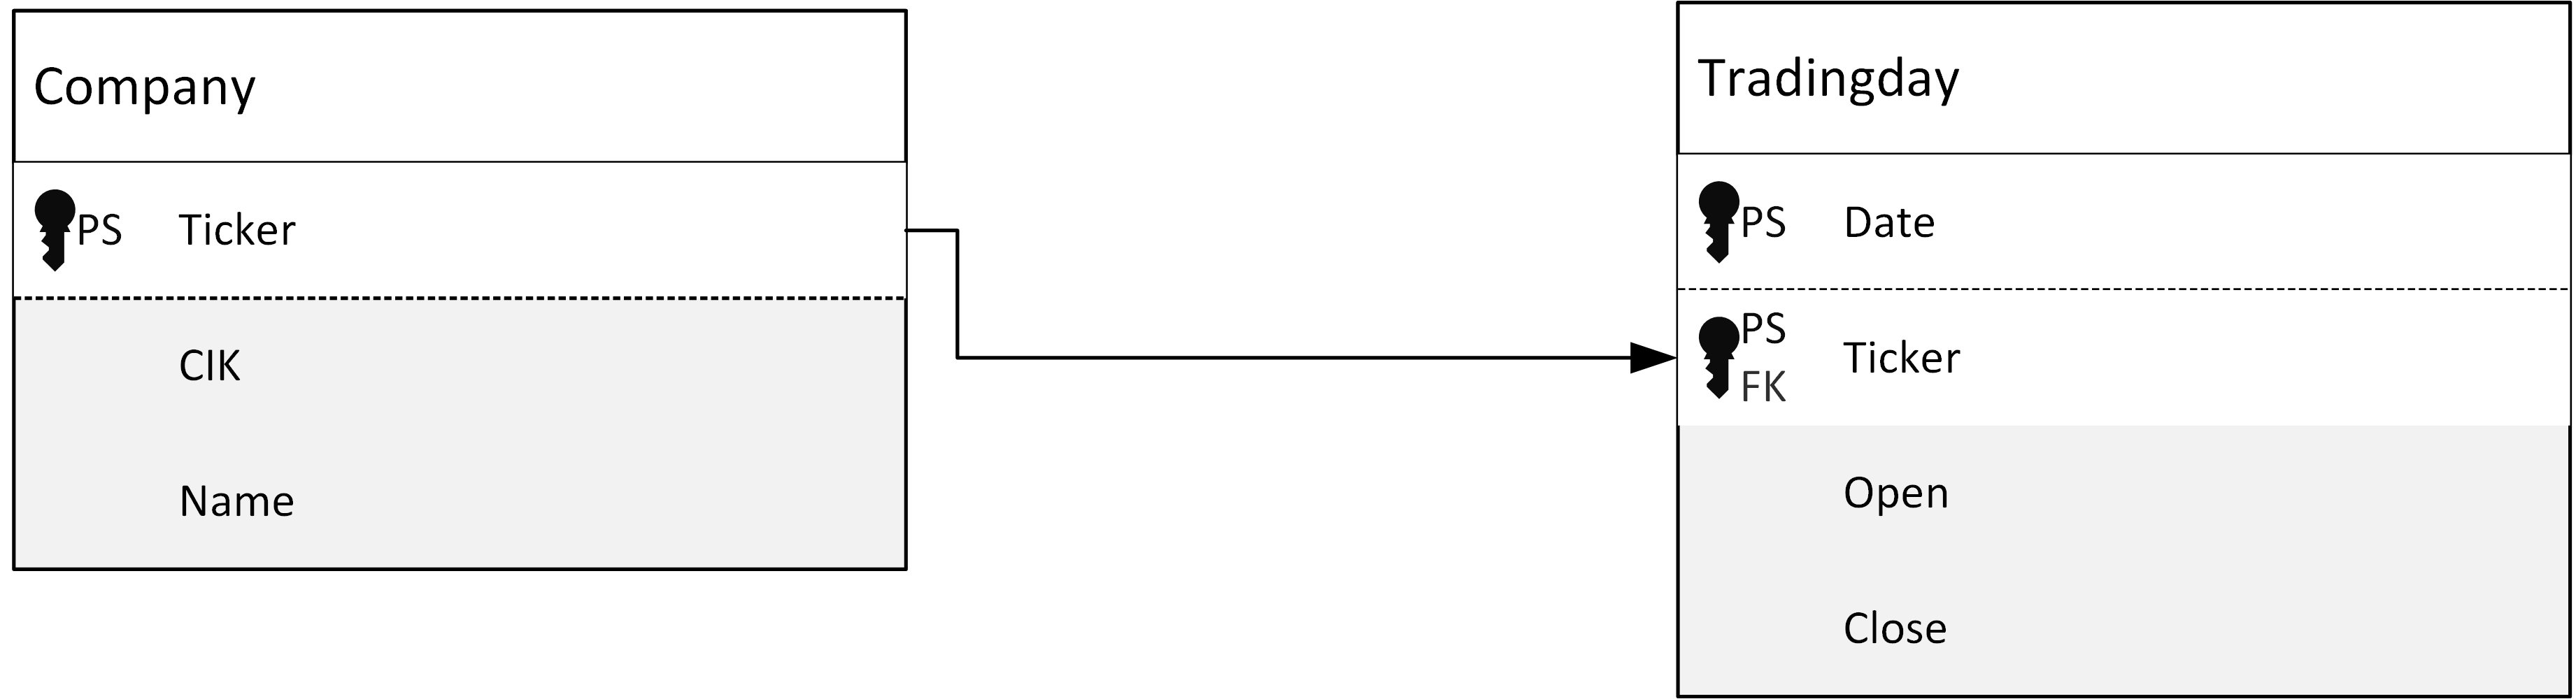
\includegraphics[width=1\textwidth]{figures/Datenmodell.png}
    \caption{Data model of the database to save the stock prices.}
    \label{figure:data_model}
\end{figure}
Since some companies became insolvent between 2003 and 2018 like Lehman Brothers Inc. in 2008 or were bought by another company like Monsanto by Bayer in 2018 and are therefore not listed on the stock anymore.
Alphavantage does not provide historic stock prices for delisted companies, therefore the reports of these companies were excluded from the research.

After this data has been loaded, the reports are indexed in two steps.
First the \ac{SRAF} index file is looped chronologically starting from the 01/01/2004.
For each entry, it is checked if the publishing company is part of the \ac{SP} 500 at the release day.
If it is, the \ac{SRAF}-specific metadata is removed from the file and the report is splitted into sentences using the sentencizer from the python package spaCy.
Since \acs{BERT} has a maximum text length it can process, it was interesting how long some of the resulting senteces were.
Bar chart \ref{figure:words_distribution} shows the distribution of different words per sentences.

\begin{figure}[h]
    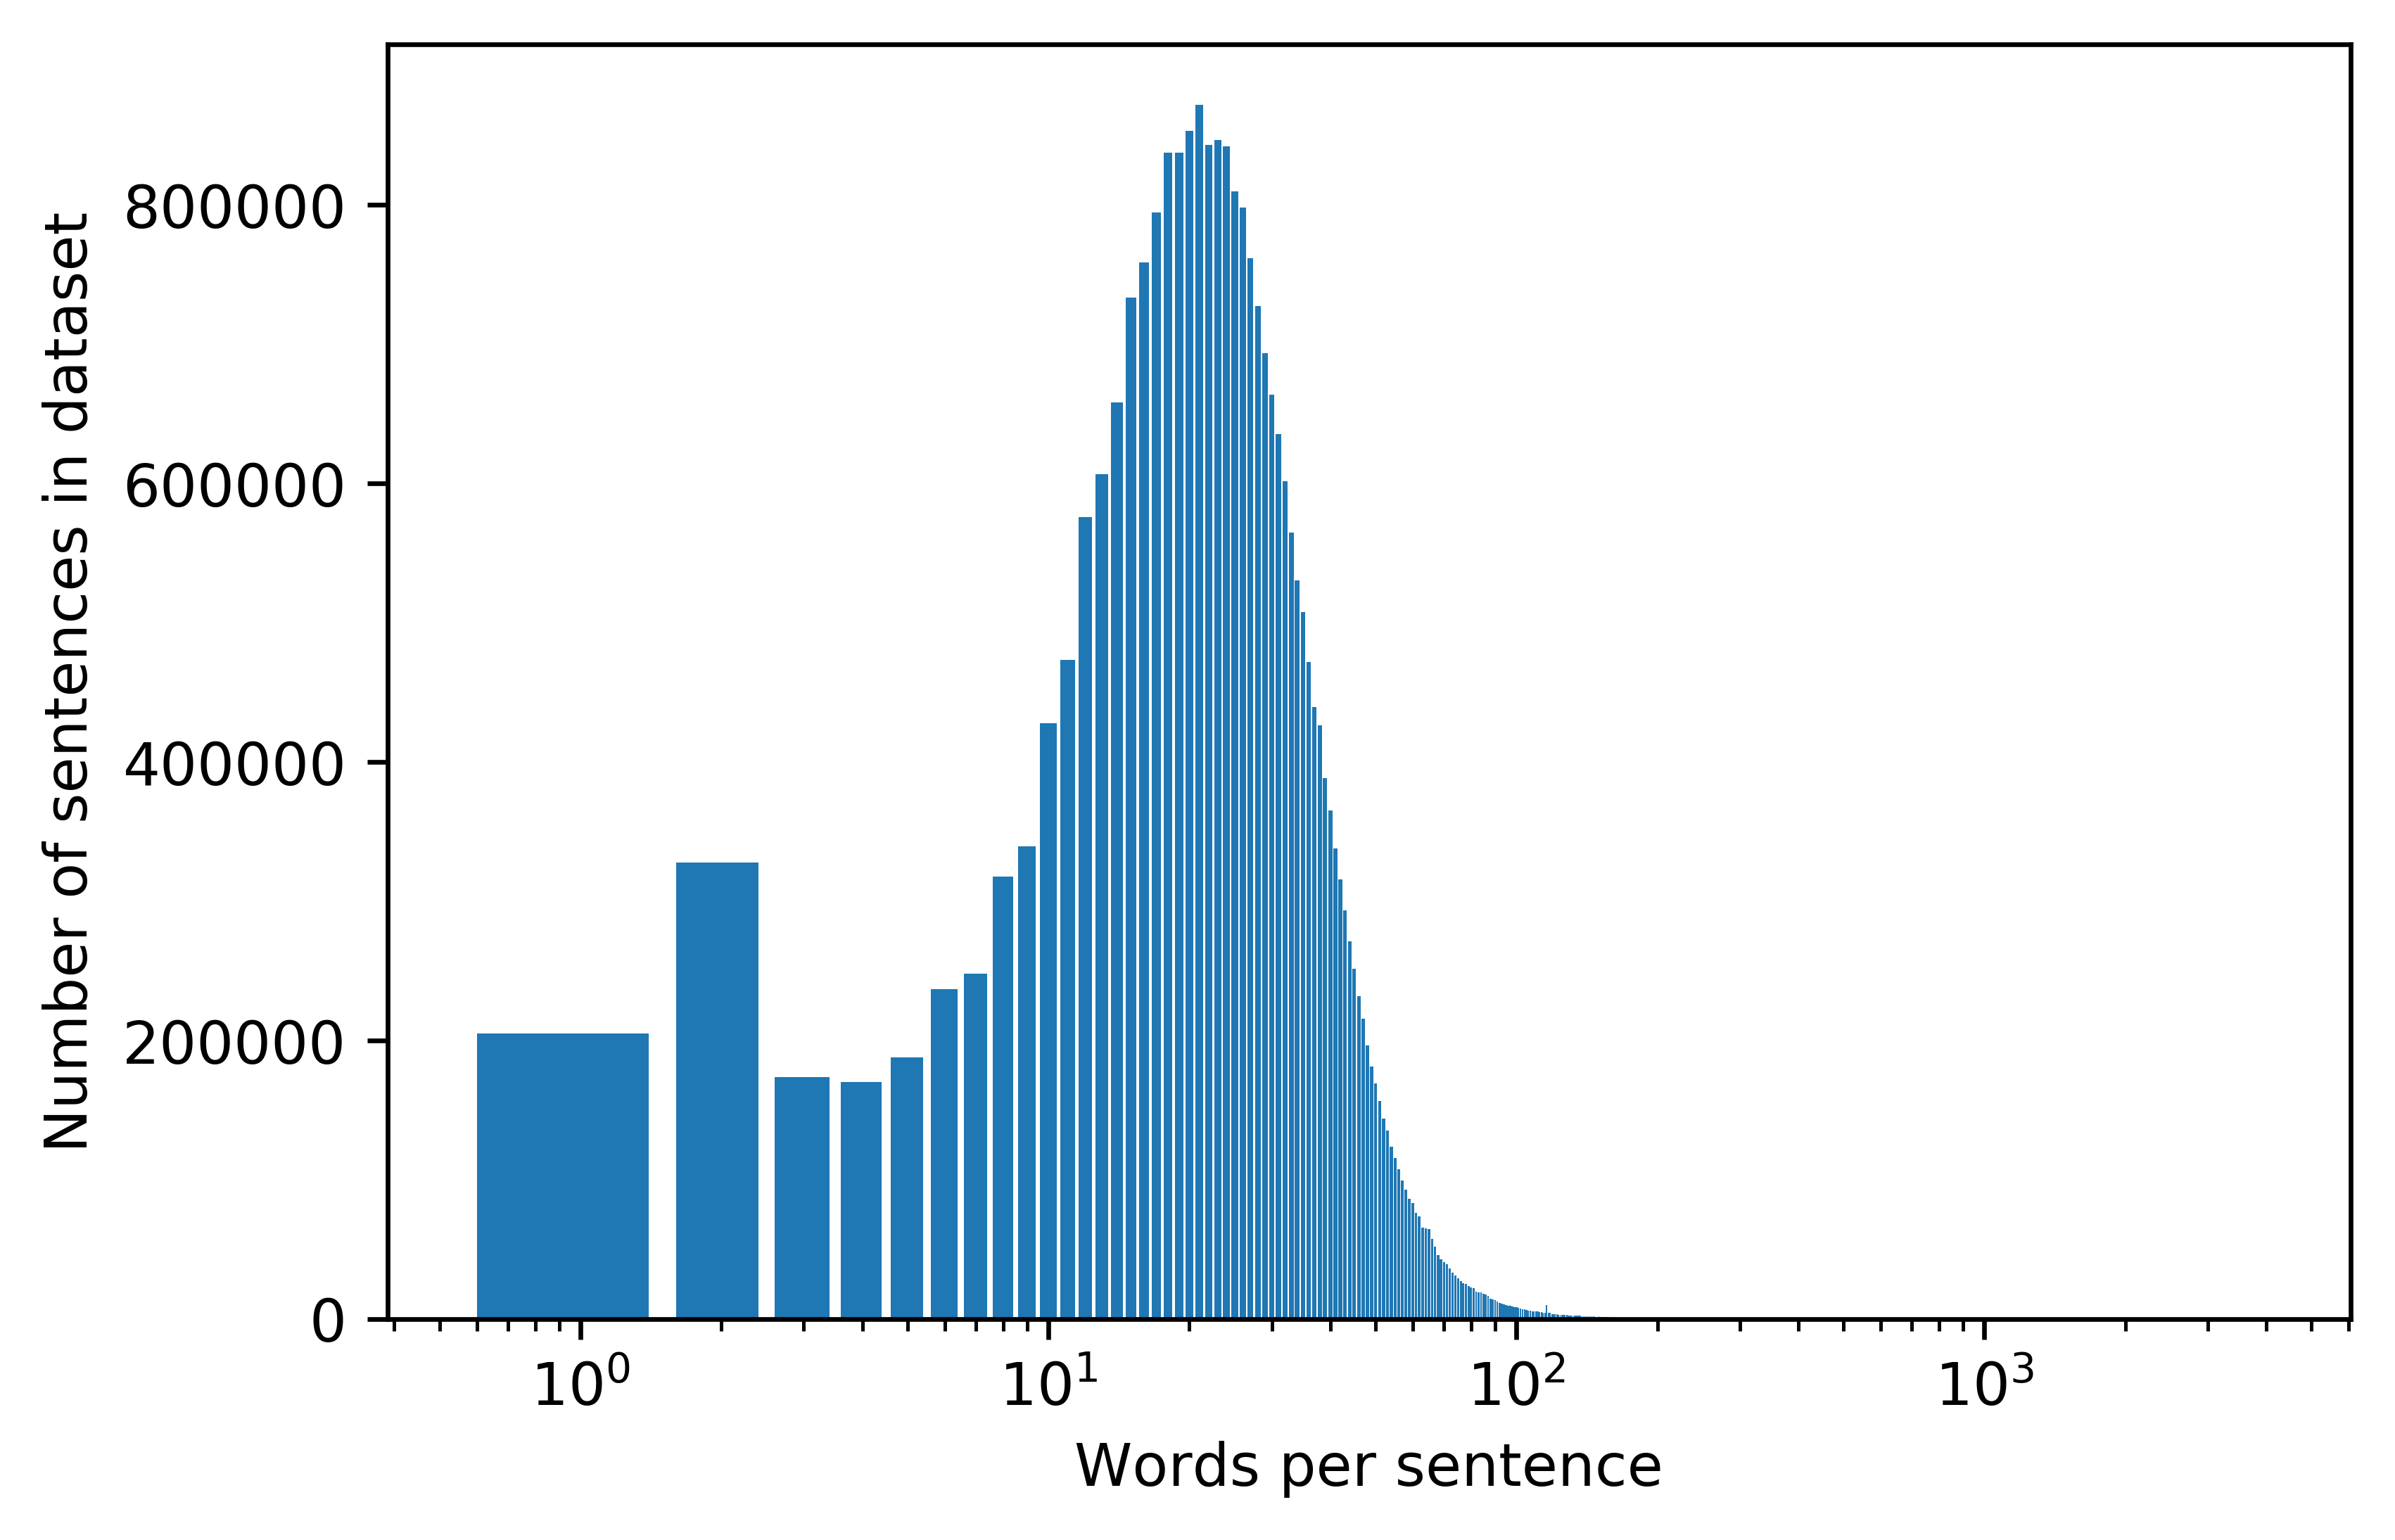
\includegraphics[width=1\textwidth]{figures/charts/words_distribution.png}
    \caption{Distribution of words per sentences.}
    \label{figure:words_distribution}
\end{figure}
% \begin{figure}[h]
%     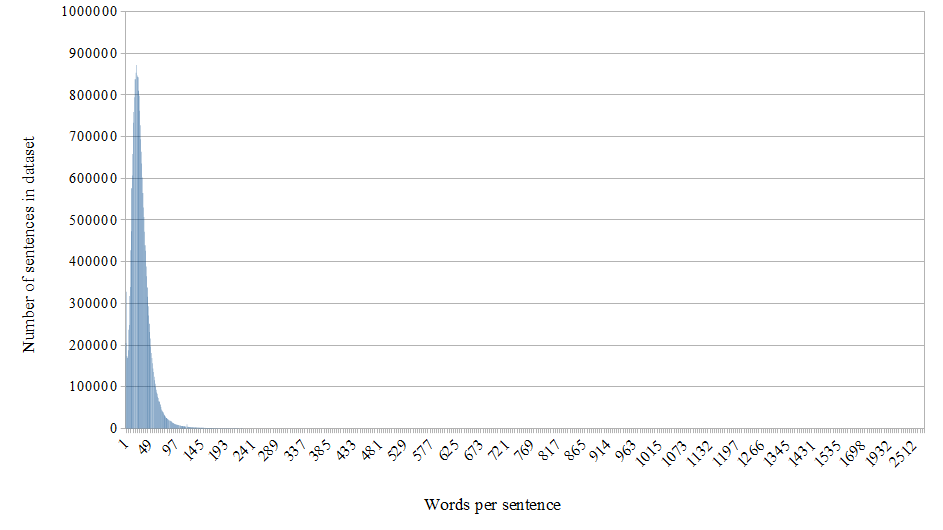
\includegraphics[width=1\textwidth]{figures/charts/words_per_sentence_distribution.png}
%     \caption{Distribution of words per sentences.}
%     \label{figure:words_distribution}
% \end{figure}
% \begin{figure}[h]
%     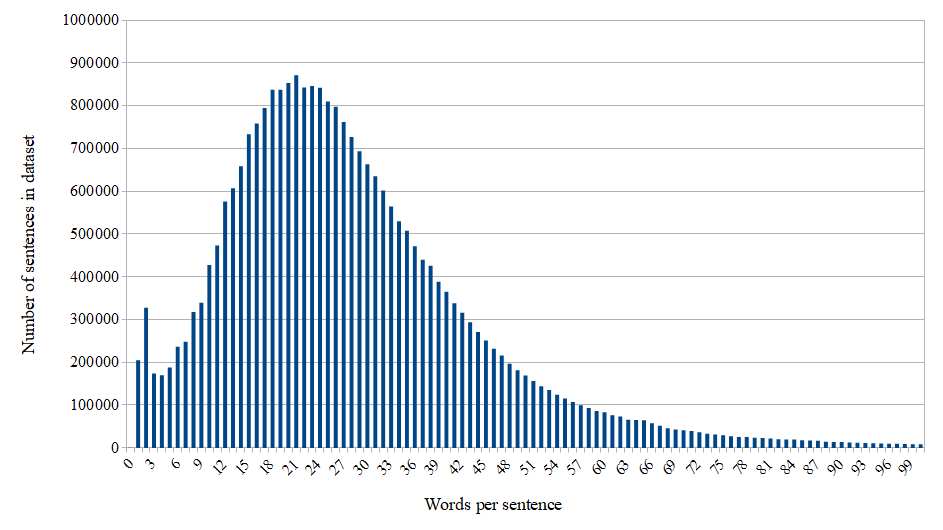
\includegraphics[width=1\textwidth]{figures/charts/words_per_sentence_distribution_0-100.png}
%     \caption{Distribution of 1 to 100 words per sentence.}
% \end{figure}

It is conspicuous, that there is a huge number of sentences with less than 8 or more than 95 words per sentence.
Sentences with less than 8 words are mostly headlines like "Item 2." or "Financial Statements and Supplementary Data Note 12.", sentences with more than 95 words are mostly regulatory texts.
Therefore these sentences were removed from the reports.
Because the whole parsing process takes two seconds per report on average, the Python multiprocessing package was used to optimize the parsing for multiple \acs{CPU}s.
Therefore the parsing of the 27562 reports took about four hours.
After this parsing is finished the resulting files are added to an index file with the company's \ac{CIK}, stock ticker symbol, filing date, form type and the file path.
The second step covers the labeling of the reports as \textit{positive} or \textit{negative}.
For that another script runs through the index file again and retrieves the price information from the database using the script in listing \ref{py:get_prices}.
\lstinputlisting[language=Python,caption={Extract from the script that labels the reports},captionpos=b, label={py:get_prices}]{listings/get_prices.py}
The highest price change of stocks happens within two days after the release of a business report \cite{Feldman2010}, therefore the limit is set to three, which also includes the day of the report release itself.
The change ratio \textit{CR} on the date \textit{d} of a company with the ticker symbol \textit{t} is then computed as following:
\begin{equation}
    CR_{d,t} = \frac{p_{close, d + 2, t} - p_{open, d, t}}{p_{open, d, t}}
\end{equation}
Whereby $p_{open, d, t}$ is the opening stock price on the day of the report release and $p_{close, d + 2, t}$ is the closing price two days after the report has been released.
If the resulting change ratio is negative the report is labeled as \textit{negative} else it is labeled as positive.
The resulting \ac{CSV} file has 24609 entries and each of these entries references one parsed report file.

